% Prosecutorial Policy Analysis — Funder Presentation
% Dvir Yogev · UC Berkeley School of Law
% February 2026

\documentclass[aspectratio=169, 11pt]{beamer}

% ---------- Theme & Colors ----------
\usetheme{metropolis}
\usepackage{appendixnumberbeamer}
\usepackage{booktabs}
\usepackage{multirow}
\usepackage{graphicx}
\usepackage{xcolor}
\usepackage{tikz}
\usepackage{tabularx}
\usepackage{array}
\usepackage{ragged2e}
\usepackage{fontspec}

% Custom colors
\definecolor{berkeleyblue}{HTML}{003262}
\definecolor{californiagold}{HTML}{FDB515}
\definecolor{foundersrock}{HTML}{3B7EA1}
\definecolor{medalistgreen}{HTML}{00B0B9}
\definecolor{alertred}{HTML}{ED4E33}
\definecolor{lightgray}{HTML}{F0F0F0}

\setbeamercolor{frametitle}{bg=berkeleyblue, fg=white}
\setbeamercolor{title}{fg=berkeleyblue}
\setbeamercolor{progress bar}{fg=californiagold}
\setbeamercolor{alerted text}{fg=alertred}
\setbeamercolor{block title}{bg=berkeleyblue, fg=white}
\setbeamercolor{block body}{bg=lightgray}
\setbeamercolor{block title alerted}{bg=alertred, fg=white}
\setbeamercolor{block body alerted}{bg=lightgray}
\setbeamercolor{block title example}{bg=medalistgreen, fg=white}
\setbeamercolor{block body example}{bg=lightgray}

\setbeamerfont{title}{size=\Large, series=\bfseries}
\setbeamerfont{frametitle}{size=\large}

% Shrink table fonts
\newcommand{\tablefont}{\fontsize{7.5}{9.5}\selectfont}
\newcommand{\smalltable}{\fontsize{6.5}{8.5}\selectfont}

% ---------- Metadata ----------
\title{Prosecutorial Policy Analysis}
\subtitle{AI-Powered Measurement of Criminal Justice Reform in California}
\author{Dvir Yogev}
\institute{Center for Law \& Justice, UC Berkeley School of Law}
\date{February 2026}

% ================================================================
\begin{document}

% ---------- TITLE ----------
\maketitle

% ---------- SLIDE: Framing — Addressing AV Feedback ----------
\begin{frame}{Thank You for the Second Look}
Last time, you raised two concerns: whether \textbf{outcome data} could support the causal questions, and whether the project was \textbf{targeted enough} toward specific causal research questions.
\vspace{6pt}

Those concerns were fair. Here is what has changed:
\vspace{6pt}
\begin{enumerate}\setlength\itemsep{6pt}
    \item \textbf{We linked outcome data and found a real signal} --- pilot results survive year fixed effects; pretrial detention shows a clean causal signal ($p_{\text{pre-trend}} = 0.90$)
    \item \textbf{We identified 6 specific causal designs} aligned to specific research questions --- each one mapped to the exact outcome data source it requires
    \item \textbf{We restructured the ask} so that each funded phase directly unlocks a specific causal study, not just more infrastructure
\end{enumerate}
\vspace{6pt}
{\small The next 15 minutes will walk you through the evidence.}
\end{frame}

% ---------- SLIDE: The Research Problem ----------
\begin{frame}{The Measurement Gap}
\begin{columns}[T]
\begin{column}{0.55\textwidth}
District Attorneys are among the \textbf{most powerful actors} in the criminal justice system, yet we lack systematic measurement of:
\begin{itemize}
    \item How their policies \textbf{vary across jurisdictions}
    \item How policies \textbf{change over time}
    \item Whether stated policy intent \textbf{affects outcomes}
\end{itemize}
\vspace{6pt}
Existing research relies on case outcomes or campaign rhetoric---neither captures the \emph{stated policy intent} that guides line prosecutors daily.
\end{column}
\begin{column}{0.42\textwidth}
\begin{alertblock}{What's Missing}
No systematic, comparable measurement of internal DA policy documents exists \textbf{anywhere}.
\end{alertblock}
\vspace{6pt}
\begin{exampleblock}{What We Built}
The first large-scale, AI-coded dataset of internal DA policy documents---infrastructure for causal inference about prosecutorial ideology.
\end{exampleblock}
\end{column}
\end{columns}
\end{frame}

% ---------- SLIDE: Data Source ----------
\begin{frame}{Data: ACLU NorCal Public Records Archive}
\begin{columns}[T]
\begin{column}{0.55\textwidth}
\textbf{2,665 internal DA policy documents} obtained by ACLU of Northern California via the California Racial Justice Act.
\begin{itemize}
    \item \textbf{41 of 58} California counties represented
    \item Charging directives, sentencing memos, diversion protocols, racial equity initiatives, bail reform orders
    \item Documents span 2015--2024
\end{itemize}
\vspace{4pt}
These are \emph{internal operating documents}---not press releases or campaign materials. They reveal what prosecutors actually tell their staff to do.
\end{column}
\begin{column}{0.42\textwidth}
\begin{block}{Why This Is Rare}
Internal policy memos are almost never publicly available. The ACLU's PRA effort created a \textbf{unique research opportunity} that may not persist indefinitely.
\end{block}
\end{column}
\end{columns}
\end{frame}

% ---------- SLIDE: The Pipeline ----------
\begin{frame}{What We Built: Research Pipeline}
\begin{center}
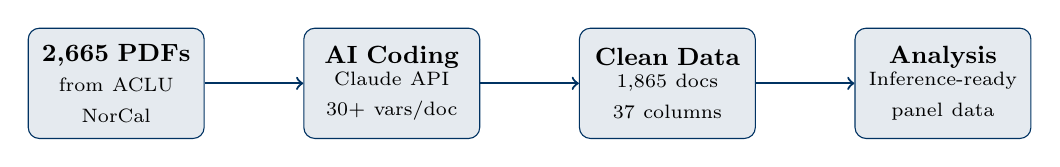
\begin{tikzpicture}[
    box/.style={rectangle, draw=berkeleyblue, fill=berkeleyblue!10, rounded corners, minimum width=2.2cm, minimum height=1.4cm, text width=2cm, align=center, font=\small},
    arrow/.style={->, thick, berkeleyblue}
]
\node[box] (a) at (0,0)   {\textbf{2,665 PDFs}\\\scriptsize from ACLU NorCal};
\node[box] (b) at (3.5,0) {\textbf{AI Coding}\\\scriptsize Claude API\\\scriptsize 30+ vars/doc};
\node[box] (c) at (7,0)   {\textbf{Clean Data}\\\scriptsize 1,865 docs\\\scriptsize 37 columns};
\node[box] (d) at (10.5,0){\textbf{Analysis}\\\scriptsize Inference-ready\\\scriptsize panel data};
\draw[arrow] (a) -- (b);
\draw[arrow] (b) -- (c);
\draw[arrow] (c) -- (d);
\end{tikzpicture}
\end{center}
\vspace{-2pt}
{\tablefont
\begin{tabularx}{\textwidth}{lX}
\toprule
\textbf{Dimension Coded} & \textbf{What's Measured} \\
\midrule
Ideological Orientation & 7-point scale: clearly progressive $\to$ clearly traditional \\
Extensive Margin & Impact on \emph{who enters} the system (charging, diversion) \\
Intensive Margin & Impact on \emph{how severely} people are treated (sentencing) \\
Specific Policies & Diversion, bail reform, enhancements, three strikes, racial justice \\
Administrative Context & New policy vs.\ continuation, DA administration \\
\bottomrule
\end{tabularx}}
\vspace{2pt}
\begin{center}\scriptsize Total API cost: \textasciitilde\$80 \quad$\cdot$\quad Processing time: \textasciitilde 2 hours\end{center}
\end{frame}

% ---------- SLIDE: Specific Policy Coding ----------
\begin{frame}{Not Just ``Progressive/Traditional'' --- We Code Specific Policies}
{\small Every document is coded on \textbf{7 specific policy dimensions}, not just a blanket ideology score.}
\vspace{3pt}
{\footnotesize
\begin{tabularx}{\textwidth}{l l X}
\toprule
\textbf{Dimension} & \textbf{Values} & \textbf{Example from Our Data} \\
\midrule
Bail position & reform / high bail & Placer: reform-oriented bail memo; SLO: bail guideline update \\
Diversion & yes / no & Sacramento, Santa Clara: explicit diversion program support \\
Enhancements & minimize / maximize & SF, LA: minimize enhancements; 6 counties maximize \\
Three strikes & restrictive / expansive & Tracked per-document across all counties \\
Racial justice & high / moderate / low & 9 counties high (post-2020 surge), 16 moderate, 10 low \\
Juvenile transfer & restrictive / expansive & 4 documents with explicit positions \\
Alt.\ to incarceration & yes / no & Whether doc endorses treatment, community service, etc. \\
\bottomrule
\end{tabularx}}
\vspace{4pt}
\begin{alertblock}{}
\textbf{This is v1.0.} Adding new dimensions (gun policy, DV protocols, immigration detainers) requires only a prompt update, not a pipeline rebuild.
\end{alertblock}
\end{frame}

% ---------- SLIDE: Face Validity ----------
\begin{frame}{Face Validity: The Pipeline Recovers Known Patterns}
{\small\color{gray} These findings build confidence that the AI coding measures real variation.}
\vspace{4pt}
\begin{columns}[T]
\begin{column}{0.48\textwidth}
\begin{block}{Gasc\'on Transformation}
LA County ideology score \textbf{tripled} under Gasc\'on\\
Cohen's $d = 0.75$, $p < 0.001$
\end{block}
\vspace{4pt}
\begin{block}{Geographic Clustering}
\begin{itemize}\setlength\itemsep{1pt}
    \item \textcolor{medalistgreen}{\textbf{Progressive:}} Sacramento $+78\%$, Yolo $+56\%$, San Diego $+50\%$
    \item \textcolor{alertred}{\textbf{Traditional:}} Stanislaus $-34\%$, Placer $-21\%$
    \item Bay Area variation: Santa Clara $+0.84$ vs Alameda $-0.15$
\end{itemize}
\end{block}
\end{column}
\begin{column}{0.48\textwidth}
\begin{block}{2020 Racial Justice Surge}
Racial justice emphasis jumped \textbf{+30pp} in one year (12\% $\to$ 42\%), tracking the post-George Floyd moment precisely.
\vspace{3pt}
Documents with high racial justice emphasis are \textbf{4.6$\times$} more likely to be progressive ($\chi^2 = 421$, $p < 0.001$).
\end{block}
\vspace{4pt}
\begin{exampleblock}{Why This Matters}
Pipeline confirms patterns any expert would expect---evidence of validity, not artifact.
\end{exampleblock}
\end{column}
\end{columns}
\end{frame}

% ---------- SLIDE: Descriptive Analysis ----------
\begin{frame}{Descriptive Analysis: Theory-Grounded Patterns}
\begin{columns}[T]
\begin{column}{0.48\textwidth}
\begin{block}{Extensive $>$ Intensive Margin}
Recent reforms disproportionately emphasize \textbf{who enters} the system (\textbf{33.9\%} extensive lenient) over \textbf{how severely} people are treated (\textbf{22.6\%} intensive lenient).
\vspace{4pt}
{\small\color{gray} Political economy logic: diversion/declination less visible to voters than sentencing leniency---safer reforms for DAs facing reelection.}
\end{block}
\end{column}
\begin{column}{0.48\textwidth}
\begin{block}{Close Elections $\to$ Progressive Policy}
Elections with margins $\leq$15pp produce \textbf{+31.2pp} more progressive policies ($p = 0.010$).
\vspace{4pt}
Continuous: $r = -0.50$ between margin and ideology ($p = 0.009$).
\vspace{4pt}
{\small\color{gray} Provides credible first stage for instrumental variables designs.}
\end{block}
\end{column}
\end{columns}
\vspace{8pt}
\begin{alertblock}{}
\textbf{Novel contributions:} The extensive-over-intensive pattern has not been documented at this scale. The election-ideology link provides the first stage for causal designs.
\end{alertblock}
\end{frame}

% ---------- SLIDE: Policy Shocks ----------
\begin{frame}{The Variation Exists: Policy Shocks = Natural Experiments}
{\small The pipeline detects sharp policy transitions---exactly the quasi-experimental variation causal designs require.}
\vspace{6pt}
\begin{columns}[T]
\begin{column}{0.48\textwidth}
\begin{block}{What We Found}
\begin{itemize}\setlength\itemsep{2pt}
    \item \textbf{9} sharp policy disruptions (2020--23)
    \item \textbf{347} novel reform adoptions tracked
    \item Progressive docs: 18\% $\to$ 56\% in 4 years
\end{itemize}
\end{block}
\vspace{4pt}
\begin{block}{Each Feature $\to$ a Causal Design}
\begin{itemize}\setlength\itemsep{2pt}
    \item 9 disruptions $\to$ \textbf{staggered DiD / event study}
    \item $\sim$5 close elections $\to$ \textbf{RDD first stage}
    \item DA transitions $\to$ \textbf{synthetic control}
    \item Margin $\to$ ideology ($r = -0.50$) $\to$ \textbf{IV}
\end{itemize}
\end{block}
\end{column}
\begin{column}{0.48\textwidth}
\begin{alertblock}{The Key Insight}
\textbf{All four pillars of modern causal inference}---DiD, RDD, synthetic control, and instrumental variables---are available in this data. No other prosecutorial dataset offers this.
\end{alertblock}
\vspace{4pt}
\begin{exampleblock}{What's Missing}
Outcome linkage (Extension 2) and geographic scale (Extension 1) to power these designs. The policy variation is already in hand.
\end{exampleblock}
\end{column}
\end{columns}
\end{frame}

% ---------- SLIDE: Jail Data Pilot ----------
\begin{frame}{Pilot Results: The Signal Is Real}
{\small Linked AI-coded policy scores to \textbf{Vera Institute Incarceration Trends} (245,840 quarterly obs., all US counties).}
\vspace{4pt}
{\tablefont
\begin{tabularx}{\textwidth}{lllX}
\toprule
\textbf{Finding} & \textbf{Estimate} & \textbf{Significance} & \textbf{Survives Controls?} \\
\midrule
Ideology $\leftrightarrow$ Jail Pop Rate & $r = -0.222$ & $p = 0.009$ & \textcolor{medalistgreen}{\textbf{Yes}} (year-demeaned) \\
Ideology $\leftrightarrow$ Jail Admissions & $r = -0.221$ & $p = 0.009$ & \textcolor{medalistgreen}{\textbf{Yes}} (year-demeaned) \\
Progressive vs Traditional & $-68.5$/100k & $d = -0.81$ & \textcolor{medalistgreen}{\textbf{Yes}} \\
LA Pretrial (Gasc\'on DiD) & $-32.1$/100k & Pre-trend $p = 0.90$ & \textcolor{medalistgreen}{\textbf{Cleanest}} \\
\bottomrule
\end{tabularx}}
\vspace{4pt}
\begin{columns}[T]
\begin{column}{0.48\textwidth}
\begin{exampleblock}{What Works}
{\small All associations \textbf{survive year fixed effects}---not a COVID artifact. Pretrial detention shows the cleanest causal signal (pre-trend $p = 0.90$). These results motivate the full-scale designs on the next slides.}
\end{exampleblock}
\end{column}
\begin{column}{0.48\textwidth}
\begin{block}{What Extensions Will Solve}
{\small Pilot $N$ is small (34 CA counties, 9 years). National expansion + case-level outcome data will power the causal designs this variation makes possible.}
\end{block}
\end{column}
\end{columns}
\end{frame}

% ---------- SLIDE: What This Can Test ----------
\begin{frame}{The Payoff: 6+ Credible Causal Studies, Ready to Run}
{\small Each row is a testable causal hypothesis. The policy variation already exists. Fund the outcome linkage.}
\vspace{4pt}
{\smalltable
\begin{tabularx}{\textwidth}{p{2.2cm}Xp{2.8cm}p{2.8cm}}
\toprule
\textbf{Policy Coded} & \textbf{Causal Question} & \textbf{Design} & \textbf{Outcome Data} \\
\midrule
Bail reform & Does reform reduce pretrial detention without increasing FTA? & Event study; DiD & Vera (\textcolor{medalistgreen}{done}); CA DOJ \\
Diversion & Do diversion memos lower recidivism? & Staggered DiD & UniCourt; CJARS \\
Declination memos & Do ``decline to prosecute'' orders lower filings? & Synthetic control & CA DOJ (\textcolor{medalistgreen}{free}) \\
Enhancement reform & Does curbing 3-strikes reduce sentence lengths? & Event study & CA Sentencing Comm. \\
Racial equity & Do equity directives reduce B/W disparities? & DiD; IV & CA DOJ by-race; CJARS \\
Close elections & Does a progressive DA \emph{cause} lower incarceration? & RDD & Vera (\textcolor{medalistgreen}{done}) \\
\bottomrule
\end{tabularx}}
\vspace{4pt}
\begin{alertblock}{}
\textbf{6 designs $\times$ multiple outcomes = a research agenda.} The policy variation is in hand. Outcome linkage (Phase 1--2) unlocks all of them.
\end{alertblock}
\end{frame}

% ---------- SLIDE: Diversion Deep Dive ----------
\begin{frame}{Deep Dive: Identifying the Causal Effect of Diversion Policies}
\begin{columns}[T]
\begin{column}{0.48\textwidth}
\begin{block}{The Question}
{\small Does adopting a diversion program \textbf{reduce recidivism} and \textbf{lower case volumes} without increasing public safety risk?}
\end{block}
\vspace{3pt}
\begin{block}{Identification Strategy}
{\small
\begin{itemize}\setlength\itemsep{2pt}
    \item \textbf{Treatment:} date a DA issues an internal diversion directive (coded by our pipeline)
    \item \textbf{Design:} staggered DiD across counties adopting at different times
    \item \textbf{Robustness:} synthetic control for Sacramento, Santa Clara
\end{itemize}}
\end{block}
\end{column}
\begin{column}{0.48\textwidth}
\begin{block}{Outcome Data Needed}
{\small
\begin{itemize}\setlength\itemsep{2pt}
    \item \textbf{CJARS:} individual trajectories---does diversion reduce $P$(re-arrest)?
    \item \textbf{UniCourt:} case outcomes---do filing rates drop? Do plea rates change?
    \item \textbf{CA DOJ:} county-level prosecution counts (free, immediate)
\end{itemize}}
\end{block}
\vspace{3pt}
\begin{exampleblock}{Why Both}
{\small CJARS = \textbf{individual mechanism}. UniCourt = \textbf{case-level detail}. Together: ``what happens to diverted people \emph{and} to case flow.''}
\end{exampleblock}
\end{column}
\end{columns}
\end{frame}

% ---------- SLIDE: Extension 1 ----------
\begin{frame}{Extension 1: Scale $\to$ Statistical Power for Causal Designs}
{\small \textbf{Right now:} 41 CA counties, $\sim$5 close elections, 6-year pre-periods. Suggestive---but underpowered for publication-quality causal inference.}
\vspace{4pt}
\begin{columns}[T]
\begin{column}{0.48\textwidth}
\begin{block}{Complete California}
\begin{itemize}\setlength\itemsep{2pt}
    \item Add \textbf{17 remaining counties} $\to$ full 58-county panel
    \item \textbf{Pre-2015 docs} $\to$ 10+ year pre-periods for event study
    \item \textbf{200-doc human validation} $\to$ publication-ready IRR
\end{itemize}
\end{block}
\end{column}
\begin{column}{0.48\textwidth}
\begin{block}{100 Largest US DA Offices}
\begin{itemize}\setlength\itemsep{2pt}
    \item \textbf{30--50 close elections} $\to$ statistically powered RDD
    \item Staggered treatment across states $\to$ robust DiD
    \item Cross-state variation $\to$ external validity
\end{itemize}
\end{block}
\end{column}
\end{columns}
\vspace{6pt}
\begin{alertblock}{What Funding Unlocks}
CA alone: $\sim$5 close elections (underpowered RDD). National expansion: \textbf{30--50 close elections}---enough for a credible regression discontinuity that can answer ``does electing a progressive DA \emph{cause} lower incarceration?''
\end{alertblock}
\end{frame}

% ---------- SLIDE: Extension 2 ----------
\begin{frame}{Extension 2: Outcome Linkage $\to$ True Causal Estimates}
{\small \textbf{Right now:} policy variation exists but is linked only to aggregate jail data (Vera). We see correlations. To make \emph{causal claims}, we need outcome data at the right resolution.}
\vspace{4pt}
\begin{columns}[T]
\begin{column}{0.48\textwidth}
\begin{block}{Aggregate $\to$ County-Level Causal}
{\tablefont
\begin{tabularx}{\columnwidth}{lX}
\toprule
\textbf{Source} & \textbf{Causal Question It Answers} \\
\midrule
CA DOJ & Do filing rates drop after ``decline to prosecute'' memos? \\
Sentencing Comm. & Do enhancement filings fall after reform? \\
Vera (\textcolor{medalistgreen}{done}) & DiD/event study on jail populations \\
\bottomrule
\end{tabularx}}
\end{block}
\end{column}
\begin{column}{0.48\textwidth}
\begin{block}{Case-Level $\to$ Mechanism Evidence}
{\tablefont
\begin{tabularx}{\columnwidth}{lX}
\toprule
\textbf{Source} & \textbf{Causal Question It Answers} \\
\midrule
UniCourt & Do diversion memos change plea bargaining? \\
CJARS & Does a diversion memo reduce $P$(prosecution $|$ arrest)? \\
\bottomrule
\end{tabularx}}
\end{block}
\end{column}
\end{columns}
\vspace{6pt}
\begin{alertblock}{What Funding Unlocks}
Without outcome linkage, we have \textbf{policy variation without a dependent variable}. Each data source above converts one row of the ``6+ causal studies'' table from potential into a publishable result.
\end{alertblock}
\end{frame}

% ---------- SLIDE: Policymaker Value ----------
\begin{frame}{Value for Policymakers}
\begin{columns}[T]
\begin{column}{0.48\textwidth}
\begin{itemize}\setlength\itemsep{6pt}
    \item \textbf{DA accountability scorecards}---comparable measures of how each office's stated policies align with its goals
    \item \textbf{Rhetoric vs.\ practice}---does a ``decline low-level drugs'' memo actually reduce drug prosecutions?
\end{itemize}
\end{column}
\begin{column}{0.48\textwidth}
\begin{itemize}\setlength\itemsep{6pt}
    \item \textbf{Benchmarking tools}---a DA considering bail reform can see how similar policies performed elsewhere
    \item \textbf{Causal evidence on the progressive prosecutor model}---answering the central question: does it work?
\end{itemize}
\end{column}
\end{columns}
\vspace{8pt}
\begin{block}{Related Work}
Felix Owusu's AV-funded project exploits two specific internal DA memos for a causal design. Our contribution scales this logic: \textbf{systematic measurement across 41+ offices and 1,865 documents}, creating variation needed for average causal effects and heterogeneity analysis.
\end{block}
\end{frame}

% ---------- SLIDE: Funding ----------
\begin{frame}[t]{Potential Funding Package}
{\small Each phase converts \textbf{potential} into \textbf{published causal evidence}. The infrastructure is built---funding buys the data and scale.}
\vspace{4pt}
\resizebox{\linewidth}{!}{%
\begin{tabular}{@{}p{0.8cm}p{3.5cm}p{1.5cm}p{1.5cm}p{3.2cm}p{3.5cm}@{}}
\toprule
\textbf{Phase} & \textbf{Components} & \textbf{Time} & \textbf{Budget} & \textbf{Causal Unlock} & \textbf{Deliverable}\\
\midrule
\textbf{1} & CA DOJ linkage; complete CA panel; human validation & 6 mo & \$45--50k & DiD + synthetic control with validated measurement & First causal estimates of DA policy effects \\[5pt]
\textbf{2} & 100 US DA offices; national election DB; CJARS app & 12--18 mo & \$100--150k & Powered RDD (30--50 elections); robust staggered DiD & National DA ideology database \\[5pt]
\textbf{3} & Case-level data (UniCourt/CJARS) & 6--12 mo & \$50--65k & IV + mechanism decomposition & Evidence of \emph{how} policy changes courtrooms \\
\bottomrule
\end{tabular}}
\vspace{4pt}

{\small \textbf{Today:} suggestive correlations (34-county pilot) $\to$ \textbf{Phase 1:} first credible causal estimates $\to$ \textbf{Phase 3:} full research program.}

{\small\textcolor{foundersrock}{\textbf{Flexible entry point:}} Phases can be combined or reordered based on priorities. For example, start with CA completion \emph{plus} CA DOJ outcome linkage (Phase 1) to test a specific causal question like diversion, while the CJARS application (Phase 2--3) proceeds in parallel.}
\end{frame}

% ---------- SLIDE: Why Now ----------
\begin{frame}{Why Fund This Now}
\begin{columns}[T]
\begin{column}{0.48\textwidth}
\begin{block}{Unique Advantages}
\begin{itemize}\setlength\itemsep{3pt}
    \item \textbf{Infrastructure is built}---pipeline, schema, analysis framework operational
    \item \textbf{Data window is closing}---ACLU PRA archive may not persist
    \item \textbf{No competitor}---no other systematic, AI-coded DA policy database exists
    \item \textbf{Pilot-tested}---demonstrated linkage to outcomes; identified the right methods
\end{itemize}
\end{block}
\end{column}
\begin{column}{0.48\textwidth}
\begin{block}{Policy Impact}
\begin{itemize}\setlength\itemsep{3pt}
    \item Answers the question \textbf{funders care about most}: do progressive reforms actually work?
    \item Enables \textbf{evidence-based evaluation} of DA accountability efforts
    \item Creates \textbf{benchmarking tools} for jurisdictions
    \item First \textbf{causal estimates} of prosecutorial policy effects
\end{itemize}
\end{block}
\end{column}
\end{columns}
\end{frame}

% ---------- SLIDE: CTA ----------
{
\setbeamercolor{background canvas}{bg=berkeleyblue}
\setbeamercolor{normal text}{fg=white}
\usebeamercolor[fg]{normal text}
\begin{frame}[plain]
\vfill
\begin{center}
{\LARGE\textbf{Let's Talk}}
\vspace{12pt}

{\normalsize \textbf{41 counties $\cdot$ 1,865 documents $\cdot$ 6+ causal designs ready to run}}
\vspace{8pt}

{\normalsize The policy variation exists. The causal signal is real.\\
Fund the outcome linkage, and this becomes a research program.}
\vspace{20pt}

{\normalsize\textbf{Dvir Yogev}}\\
{\small Post-Doctoral Researcher $\cdot$ UC Berkeley School of Law}\\
{\small\textcolor{californiagold}{dyo@berkeley.edu}}
\vspace{12pt}

{\scriptsize\textcolor{californiagold}{github.com/dyo2112/prosecutor-policies-causal-inference}}\\
{\scriptsize Full pilot report, figures, and replication code available in repository}
\end{center}
\vfill
\end{frame}
}

% ================================================================
% BACKUP SLIDES
% ================================================================
\appendix

{
\setbeamercolor{background canvas}{bg=berkeleyblue!90}
\setbeamercolor{normal text}{fg=white}
\usebeamercolor[fg]{normal text}
\begin{frame}[plain]
\vfill
\begin{center}
{\Large\textbf{Additional Detail}}
\end{center}
\vfill
\end{frame}
}

% ---------- BACKUP: Overcoming Limitations ----------
\begin{frame}{Overcoming Pilot Limitations}
\resizebox{\linewidth}{!}{%
\begin{tabular}{p{3.5cm}p{4.5cm}p{6cm}}
\toprule
\textbf{Limitation} & \textbf{Root Cause} & \textbf{Solution} \\
\midrule
COVID confounds DiD & All CA counties declined in 2020 & Multi-state data; synthetic control \\[6pt]
Parallel trends violated & LA converging pre-Gasc\'on & Longer pre-period + case-level data \\[6pt]
TWFE non-significant & 34 counties, 9 years & National expansion increases $N$ \\[6pt]
Aggregate data too coarse & Cannot distinguish mechanisms & Case-level data from CJARS \\
\bottomrule
\end{tabular}}
\end{frame}

% ---------- BACKUP: Causal Strategies ----------
\begin{frame}{Causal Identification Strategies}
\resizebox{\linewidth}{!}{%
\begin{tabular}{p{3cm}p{4cm}p{4cm}p{3cm}}
\toprule
\textbf{Design} & \textbf{Current Status} & \textbf{What's Needed} & \textbf{Extension} \\
\midrule
RDD & $\sim$5 close CA elections & 30--50 close elections & Ext 1 (national) \\[6pt]
Stacked DiD & 9 disruptions; Vera only & More outcomes + transitions & Ext 1 + 2 \\[6pt]
Synthetic Control & Gasc\'on pilot works & More outcome data & Ext 2 \\[6pt]
Event Study & 6-year pre-period & Longer pre-period & Ext 1 \\[6pt]
IV & Margin $\to$ ideology ($r = -0.50$) & Outcome data for 2nd stage & Ext 2 \\
\bottomrule
\end{tabular}}
\end{frame}

% ---------- BACKUP: Extension 2 Detail ----------
\begin{frame}{Outcome Data Sources (Detail)}
\resizebox{\linewidth}{!}{%
\begin{tabular}{p{3cm}p{5cm}lrl}
\toprule
\textbf{Source} & \textbf{Records} & \textbf{Timeline} & \textbf{Cost} & \textbf{Priority} \\
\midrule
CA DOJ OpenJustice & County-yr arrest, filing, incarceration & Immediate & Free & High \\[6pt]
CA Sentencing Comm. & Enhancement filings, 3-strikes & 1--2 mo & Free & High \\[6pt]
Vera (done) & Quarterly jail pop and admissions & Done & Done & Done \\[6pt]
UniCourt / PACER & Case dispositions, plea bargains & 2--3 mo & \$30--50k & Very high \\[6pt]
CJARS & Arrest $\to$ parole, 24 states & 3--12 mo & \$5k & Highest \\
\bottomrule
\end{tabular}}
\vspace{8pt}

{\small\textbf{Case-level data is the gold standard:} it links policy documents directly to line-prosecutor behavior.}
\end{frame}

% ---------- BACKUP: Disruption Detection ----------
\begin{frame}{Policy Disruption Detection: Methodology}
\resizebox{\linewidth}{!}{%
\begin{tabular}{lrp{8cm}}
\toprule
\textbf{Signal} & \textbf{Weight} & \textbf{Method} \\
\midrule
Ideology Velocity & 30\% & Rate of ideology change vs.\ prior 2-year baseline \\[6pt]
Novelty Index & 25\% & Proportion of first-time policy types \\[6pt]
Topic Shift & 20\% & Jensen-Shannon divergence of topic distributions \\[6pt]
Margin Reversal & 15\% & Flips in extensive/intensive leniency direction \\[6pt]
DA Transition & 10\% & New administration detection \\
\bottomrule
\end{tabular}}
\vspace{8pt}

{\small\textbf{Top disruptions:} SF 2020 (Boudin, 0.572), LA 2021 (Gasc\'on, 0.549), Sacramento 2022 (0.412)}
\end{frame}

% ---------- BACKUP: Anticipated Objections (1/2) ----------
\begin{frame}{Anticipated Objections (1/2)}
\begin{block}{``Policy changes aren't random. Where's the identification strategy?''}
{\small (1)~\textbf{Close elections are as-good-as-random}---RDD at 50\% cutoff; national expansion gives 30--50 races. (2)~\textbf{Election margin is an IV}---$r = -0.50$ with ideology. (3)~\textbf{Memo timing is plausibly exogenous}---the exact date a DA issues a specific memo has quasi-random administrative variation; staggered DiD exploits this. (4)~\textbf{Synthetic control} needs parallel trends, not randomization---LA pilot: $p_{\text{pre-trend}} = 0.90$. (5)~\textbf{Triangulation}: when all four designs agree, combined evidence is strong.}
\end{block}
\vspace{6pt}
\begin{block}{``Policy documents $\neq$ practice. How do you know memos change anything?''}
{\small That's why Extension 2 is Priority 1. We test whether ``diversion-positive'' memos predict more diversions. Even the stated-policy variation is \emph{itself} a novel descriptive contribution.}
\end{block}
\end{frame}

% ---------- BACKUP: Anticipated Objections (2/2) ----------
\begin{frame}{Anticipated Objections (2/2)}
\begin{block}{``You only have California. Isn't this just a Blue State story?''}
{\small That's the point of Extension 1. CA has internal variation (Bay Area vs.\ Central Valley), but external validity requires the 100 largest DA offices nationally.}
\end{block}
\vspace{6pt}
\begin{block}{``AI coding isn't reliable enough for research.''}
{\small Face validity is strong ($d = 0.75$ on Gasc\'on, geographic clustering matches expectations). Phase 1 includes 200-doc human validation for gold-standard IRR. Pipeline cost: \$80, runtime: 2 hours.}
\end{block}
\end{frame}

\end{document}
